\chapter{Proces}
\index{Proces}
\label{proces}

Dit hoofdstuk beschrijft het ontwikkelproces van deze stage. Hierbij zal de manier van werken centraal staan, alswel het verloop.

\section{Projectmanagement}
\index{projectmanagement}

Zoals in het Plan van Aanpak vermeld staat (in het de paragraaf fasering op bladzijde \pageref{fasering}), is binnen Delem elk project opgedeeld in zogenaamde \index{Milestones}\emph{milestones}. Voor dit project is elke milestone weer opgedeeld in zogenaamde \index{Increments}\emph{increments}, een periode van twee weken. Hierbij stond elke increment een hoofdfeature centraal. Dit zal in de overzichten op de pagina's hierna te zien zijn.

Dit is te vergelijken met het standaard \index{waterval model}waterval model:

\begin{figure}[h]
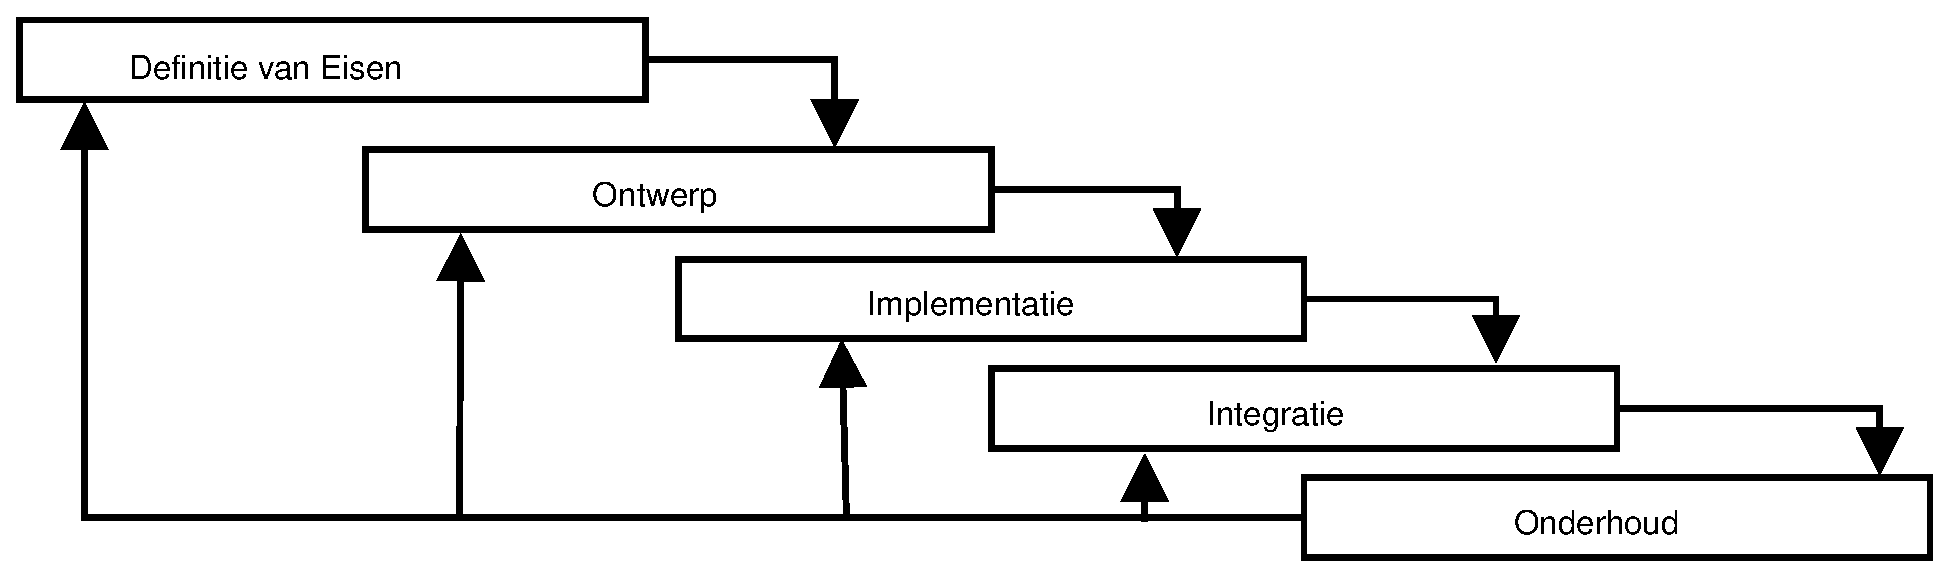
\includegraphics[width=\textwidth]{waterval}
\end{figure}

Het grootste verschil met het standaard waterval model, is dat nu het model meerdere keren doorlopen wordt (namelijk \'e\'en waterval per increment). Verder wordt aan het begin van elke increment naar de requirements gekeken, in tegenstelling tot eenmalig aan het begin van het project. Tenslotte is de terugkoppeling met de gebruikers iets waarin het 'standaard' watervalmodel helemaal niet voorziet.

\section{Besprekingen}
\index{Besprekingen}

Na een gesprek met de bedrijfsbegeleider, besloten we elke maandag een uur te vergaderen over het project. Hierbij stonden de volgende zaken centraal:

\begin{itemize}
\item Voortgang \\
Wat is er van de zaken die vorige keer besproken zijn terecht gekomen?
\item Toekomst \\
Wat is de bedoeling voor volgende weken?
\end{itemize}

Deze aanpak is gekozen, omdat de uiteindelijke \index{requirements}requirements van het project (dus een concrete lijst wat het moet kunnen) niet beschikbaar was. Vanuit Delem was het idee om ontwikkelaars het programma te laten gebruiken en aan de hand van het commentaar erop het te laten groeien. Zo kwam er een programma precies volgens de wensen van de ontwikkelaars (dit is prima omdat het voor intern gebruik is)

Na elke increment is er gekeken naar wat we nu hadden en wat de bedoeling was om eraan toe te voegen. Zo kwam er op de uiteindelijke planning naar voren dat er halverwege increment 6 weinig meer aan toe te voegen was, omdat er geen nieuwe requirements waren die ge\"\i mplementeerd moesten worden.

Om het verloop zo goed mogelijk weer te geven, is er op de volgende bladzijde de initi\"ele planning te zien en op de bladzijde daarna het definitieve resultaat van de planning.

\begin{landscape}

\section{Initi\"ele Planning}
\index{Planning!Initi\"ele}

Dit is de initi\"ele planning. Kenmerkend is, dat er weinig vooruit gepland is, omdat we niet teveel op de zaken vooruit wilden lopen. Dit omdat er in dit stadium weinig bekend was over de gewenste functionaliteit.

\begin{figure}[h]
%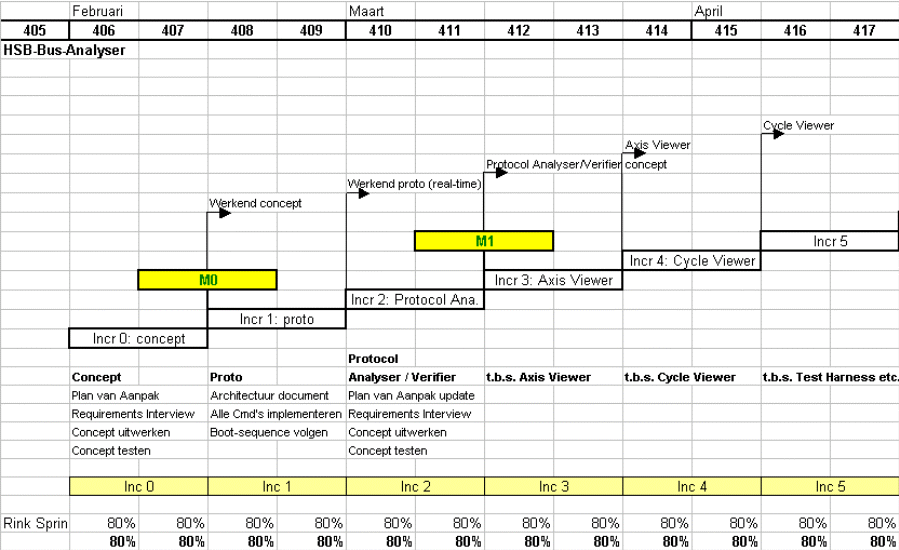
\includegraphics[width=20cm,height=9.5cm]{initiele_planning.png}
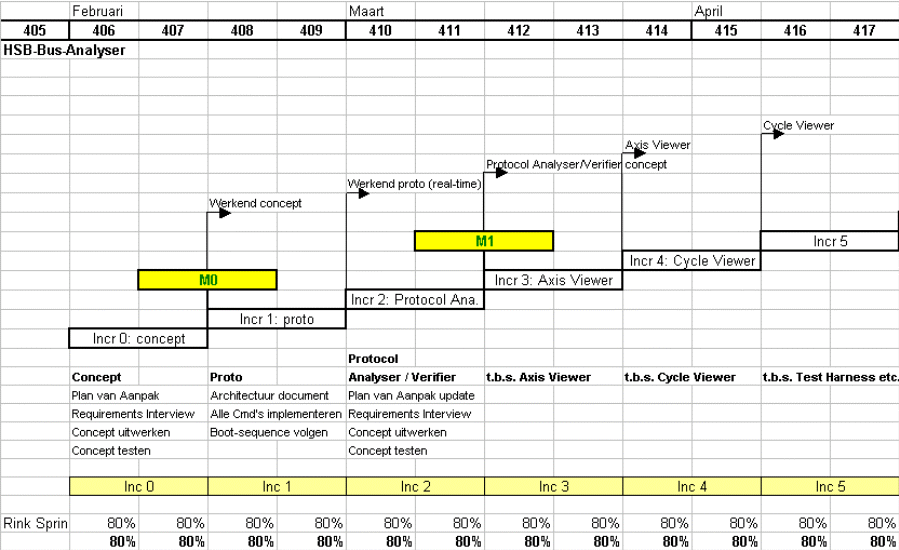
\includegraphics[width=15cm]{initiele_planning.png}
\end{figure}

\newpage

\section{Definitieve Resultaat}
\index{Resultaat!Definitieve}

Uiteindelijk is dit de realiteit geworden. Kenmerkend is, dat bijvoorbeeld de hele Cycle Viewer increment eruit gevallen is, omdat achteraf bleek dat de persbesturing deze functionaliteit al bevatte.

\begin{figure}[h]
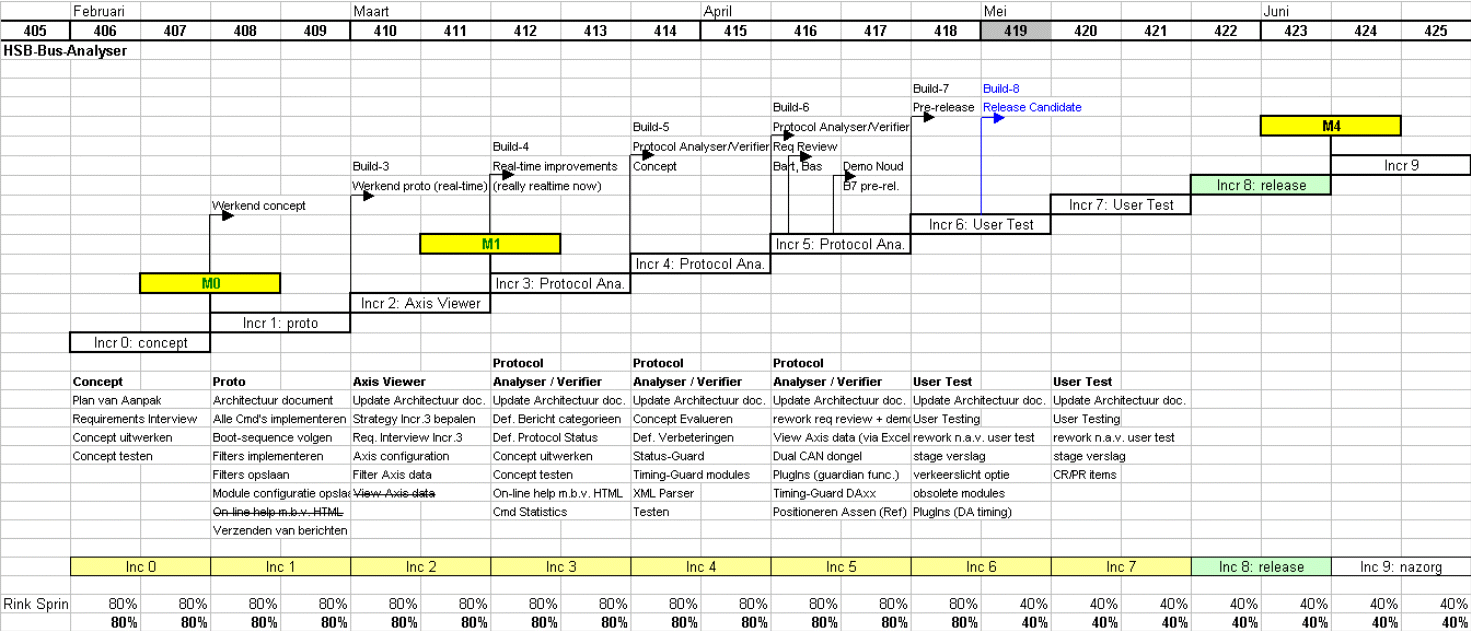
\includegraphics[width=20.9cm,height=9.7cm]{def_res.png}
\end{figure}

\end{landscape}
